\section{Graph Databases}
\label{sec:prelim-db-graph}

\todo{$\intro*\underlying{\gamma}$ and ""underlying graph""}

For a detailed introduction to "CRPQs", the reader can also
see \cite{Figueira2020Containment21Foundations}.
For a more general introduction to different query languages for "graph databases"---including "CRPQs"---see \cite{Barcelo2013Querying}, and for a more practical approach,
see \cite{AnglesEtal2017Foundations}.

\subsection{Conjunctive Regular Path Queries}

\Cref{sec:prelim-db-relational} shows that "conjunctive queries"---and "unions
thereof@UCQ"---is a reasonable query language: it is expressive enough to capture
many of the queries that are written in practice in SQL, but small enough
to be amenable to static analysis thanks to "duality@@CQ".
However, "conjunctive queries", and in fact the larger language
of "first-order logic", or \emph{relational calculus},
is remarkably powerless against ``graph-traversal queries''.

\begin{figure}[h]
    \centering
    \begin{tikzpicture}
        	\node (a1) {author$_1$};
	\node (p1) [below right=1cm and 0cm of a1] {paper$_1$};
	\node (a2) [above right=1cm and 0cm of p1] {author$_2$};
	\node (p2) [below right=1cm and 0cm of a2] {paper$_2$};
	\node (a3) [above right=1cm and 0cm of p2] {author$_3$};
	\node (a4) [right = 1cm of a3] {author$_4$};
	\node (p3) [below right=1cm and 0cm of a4] {paper$_3$};
	\node (a5) [above right=1cm and 0cm of p3] {author$_5$};

	\draw[wrote,edge] (a1) edge node[fill=white] {\footnotesize wrote} (p1)
		(a2) edge node[fill=white] {\footnotesize wrote} (p1)
		(a2) edge node[fill=white] {\footnotesize wrote} (p2)
		(a3) edge node[fill=white] {\footnotesize wrote} (p2)
		(a4) edge node[fill=white] {\footnotesize wrote} (p3)
		(a5) edge node[fill=white] {\footnotesize wrote} (p3);
	\draw[advised,edge] (a4) edge node[fill=white, yshift=1em] {\footnotesize advised} (a3)
		(a5) edge node[fill=white, yshift=1em] {\footnotesize advised} (a4);
    \end{tikzpicture}
    \caption{%
        \AP\label{fig:example-graph-database}%
        A "relational database" with two binary "predicates".
    }
\end{figure}
We illustrate this idea on a simplified example---to see a real example,
see \Cref{fig:sparql,fig:example-wikidata,tab:output-sparql,fig:intro-SPARQL-as-CRPQ}.
We depict in \Cref{fig:example-graph-database} a "relational database"
over the "purely relational signature" with two binary "predicates"
$\atom{\wrote}$ and $\atom{\advised}$. Vertices of the "structure"
represent people, and an edge $x \atom{\wrote} y$ indicate
that the person $x$ wrote the paper $y$, while edges $x \atom{\advised} y$
indicate that person $x$ was the Ph.D. advisor of person $y$.
While "conjunctive queries" can express properties like
\[
    \gamma_1(x, y) = x \atom{\wrote} z
        \land y \atom{\wrote} z,   
\]
that asks for all pairs of co-authors, it cannot express transitive-based
properties; in fact, even the full "first-order logic" cannot express such properties.
\begin{proposition}
    \label{prop:fo-no-trans}
    There is not "first-order formula" $\gamma_2(x,y)$
    that ouputs all pairs "st" $x$ is a scientific ancestor of $y$---"ie"
    "st" there is a non-empty path from $x$ to $y$ that only consists
    of $\advised$ edges.
\end{proposition}

\begin{proof}
    Assume by contraction that this would be the case. Clearly, $\gamma_2(x,y)$
    is closed under "homomorphisms", and so by "Rossman's theorem",
    it would be equivalent to a "UCQ", say
    $\delta_1(x,y) \lor \dotsc \lor \delta_k(x,y)$.
    We let $n$ be strictly greater than the "diameter" of any $\delta_i$,
    and define $\tup{\?P_n,p_0,p_n}$ to be the "pointed relational database"
    consisting the facts
    \[
        p_0 \atom{\wrote} p_1 \atom{\wrote} \dotsc \atom{\wrote} p_n,
    \]
    which is actually a shorthand for
    \[
        \{p_0 \atom{\wrote} p_1,\; p_1 \atom{\wrote} p_2,\;
        \dotsc,\;p_{n-1} \atom{\wrote} p_n\}.
    \]
    Then clearly, $\tup{\?P_n,p_0,p_n} \FOmodels \gamma_2(x,y)$
    and so $\tup{\?P_n,p_0,p_n} \FOmodels \delta_i(x,y)$ for some $i\in \intInt{1,k}$.
    By "duality@@CQ", there exists a "homomorphism" from the "canonical database@@cq"
    $\tup{\?D_i,x,y}$ of $\delta_i(x,y)$ to $\tup{\?P_n,p_0,p_n}$.
    However, the "distance@@struct" from $x$ to $y$ in $\?G_i$ is strictly
    upper bounded by $n$, since $n$ was chosen to be
    strictly greater than the "diameter" of $\?D_i$, and the distance from $x$ to $y$
    is exactly $n$.
    Since "homomorphisms" contract distances, we have reached a contradiction.
    And hence, the property of \Cref{prop:fo-no-trans} is not "first-order definable".%
    \footnote{A much more common way of proving \Cref{prop:fo-no-trans} is by using the notion
    of Ehrenfeucht–Fraïssé games, see "eg" \cite[Proposition~2.3.28]{Kolaitis2007FiniteModelTheory}.
    or Gaifman/Hanf-locality, see "eg" \cite{Barcelo2009Locality}.
    In all cases, the proof relies on an idea that "first-order queries" are local.
    In our proof, the notion of locality---formalized by the fact that "homomorphisms" contract
    the "distances@@struct"---is extremely strong, but is only valid over the "first-order queries"
    amenable to "duality@@CQ", "ie" "UCQs". This results in a very simple proof,
    which however relies on a highly non-trivial result, namely "Rossman's theorem".
    On the other hand, a proof based on Ehrenfeucht–Fraïssé games or
    Gaifman/Hanf-locality does not rely on any deep theorem, but the notion of
    locality it manipulates is much more complex, as it captures all "first-order queries".}
\end{proof}

Queries such as the one of \Cref{prop:fo-no-trans} do not arise
over all kinds of databases: for instance, 
transitive closures of tables---or of projections of table---
for \Cref{fig:relational-database-cinema} would not make any sense.
On the other hand, it is a very natural construction
for databases such as the ones of \Cref{fig:example-graph-database,fig:example-wikidata}.
Transitive closures naturally arise in databases whose nodes are homogeneous,
and in particular for human-centered data---see for instance \cite{Neo4jPanama}.
Rather than encoding this kind of data into "relational databases",
by inferring from the examples of \Cref{fig:example-graph-database,fig:example-wikidata},
we model "graph databases" as edge-labelled directed graphs, or equivalently
as "relational structures" over a finite "signature" consisting only of
binary "predicates".
\AP Formally, given an alphabet $\?A$, a ""graph database"" over $\?A$
consists of a pair \AP$\?G = \tup{G, \edges{G}}$,
where $\intro*\edges{G} \subseteq \vertex G \times \A \times \vertex G$
is a set of labelled edges---sometimes also called atoms.

This definition was motivated by the need to have database models
centred around the notion of paths.
We then naturally extend the language of "conjunctive queries"
to allow for path navigation: this is done by allowing these queries
to ask for the existence of a \emph{path} between two variables
labelled by a given regular language. For instance,
$x \atom{ (ab)^*} y$ asks that there is path from $x$
to $y$ that alternates between $\atom{a}$ and $\atom{b}$ edges.

\begin{definition}[CRPQ: syntax]
    A \AP""conjunctive regular path query"", or \reintro{CRPQ} for short,
    $\gamma(\bar x)$ over $\A$ consists
    of a set of triples $\tup{y,L,z}$ together with a tuple of variables $\bar x$,
    where $L$ is a "regular language" over $\A$, and $y$ and $z$ are variables.
    We denote by \AP$x \intro*\atom{L} y$ the triple $\tup{x,L,y}$,
    called ""atom"". The set $\intro*\atoms{\gamma}$ of "atoms" is denoted conjunctively.
    We denote by $\vars{\gamma}$ the set of variables occurring in $\gamma$. As for
    "CQs", variables of $\bar x$ are called \reintro{output variables}.
\end{definition}

An example of "conjunctive regular path query" is 
\[
    \gamma_3(x, y) \defeq x \atom{\wrote} z
        \land z' \atom{\wrote} z 
        \land y \atom{({\advised})^*} z',
\]
which intuitively asks for, in a given "graph databases",
all pairs of people $\tup{x,y}$ such that
\begin{itemize}
    \item $x$ has written some paper $z$, and some person $z'$ also wrote $z$,
    \item this $z'$ can be reached from $y$ by taking an arbitrary sequence
        of $\atom{\advised}$ edges.
\end{itemize}
Reformulating the constraints, we get that $x$ and $z'$ should be co-authors,
and that $z'$ should be a scientific descendant---in the broad sense---of $y$.
Hence, the query asks for all pairs $\tup{x,y}$ "st" $x$ is a co-author of a
``scientific descendant'' of $y$.

By definition, "conjunctive regular path queries" over $\A$ can be seen
as "finite@@struct" "pointed structures" over the infinite "signature"
$\intro*\signatureCRPQ{\A}$ that has a binary "predicate" $\atom{L}$ for each "regular language"
$L \subseteq \A^*$: this leads to a natural depiction of these
queries, see \Cref{fig:prelim-db-crpq-as-struct}.
\begin{marginfigure}
    \centering
    \begin{tikzpicture}
        \node[vertex] at (0,0) (x) {};
\node[vertex, below right=1cm and .5cm of x] (z) {};
\node[vertex, above right=1cm and .5cm of z] (z') {};
\node[vertex, right=1.5cm of z'] (y) {};

\node[above=2pt of x] {$x$};
\node[above=2pt of y] {$y$};

\draw[edge, wrote]
	(x) edge node[fill=white, xshift=-.2em] {\footnotesize wrote} (z)
	(z') edge node[fill=white, xshift=.2em] {\footnotesize wrote} (z);
\draw[edge, advised]
	(y) edge[bend right] node[fill=white, yshift=1em] {\footnotesize advised${}^*$} (z');
    \end{tikzpicture}
    \caption{\AP\label{fig:prelim-db-crpq-as-struct} Graphical representation
    of the "CRPQ" $\gamma_3(x,y)$.}
\end{marginfigure}

\begin{definition}[CRPQ: semantics]
    Given a "CRPQ" $\gamma(\bar x)$ and a "pointed graph database"
    $\tup{\?G,\bar u}$, an \AP""evaluation map"" from $\gamma(\bar x)$
    to $\tup{\?G, \bar u}$ is a function from $\vars{\gamma}$ to $G$
    that sends $\bar x$ to $\bar u$, and such that for every
    atom $x \atom{L} y$ of $\gamma$, there exists a path from $f(x)$ to
    $f(y)$ in $\?G$ labelled by some word of $L$. See \Cref{fig:prelim-db-evaluation-map}
    for an example.%

    When such an "evaluation map" exists, we say that $\tup{\?G,\bar u}$
    \AP""satisfies@@db"" $\gamma(\bar x)$, which we still denote by
    $\tup{\?G,\bar u} \reintro*\FOmodels \gamma(\bar x)$
    or $\bar u \in \reintro*\semFO{\gamma(\bar x)}{\?G}$.
    The set $\semFO{\gamma(\bar x)}{\?G}$ is called the ""evaluation""
    of $\gamma(\bar x)$ over $\?G$.
\end{definition}

\begin{figure}
    \centering
    \begin{tikzpicture}
        % Query
        \begin{scope}[xshift=2cm]
            \node[vertex] at (0,0) (x) {};
\node[vertex, below right=1cm and .5cm of x] (z) {};
\node[vertex, above right=1cm and .5cm of z] (z') {};
\node[vertex, right=1.5cm of z'] (y) {};

\node[above=2pt of x] {$x$};
\node[above=2pt of y] {$y$};

\draw[edge, wrote]
	(x) edge node[fill=white, xshift=-.2em] {\footnotesize wrote} (z)
	(z') edge node[fill=white, xshift=.2em] {\footnotesize wrote} (z);
\draw[edge, advised]
	(y) edge[bend right] node[fill=white, yshift=1em] {\footnotesize advised${}^*$} (z');
        \end{scope}

        % Graph
        \begin{scope}[yshift=-3cm]
            	\node (a1) {author$_1$};
	\node (p1) [below right=1cm and 0cm of a1] {paper$_1$};
	\node (a2) [above right=1cm and 0cm of p1] {author$_2$};
	\node (p2) [below right=1cm and 0cm of a2] {paper$_2$};
	\node (a3) [above right=1cm and 0cm of p2] {author$_3$};
	\node (a4) [right = 1cm of a3] {author$_4$};
	\node (p3) [below right=1cm and 0cm of a4] {paper$_3$};
	\node (a5) [above right=1cm and 0cm of p3] {author$_5$};

	\draw[wrote,edge] (a1) edge node[fill=white] {\footnotesize wrote} (p1)
		(a2) edge node[fill=white] {\footnotesize wrote} (p1)
		(a2) edge node[fill=white] {\footnotesize wrote} (p2)
		(a3) edge node[fill=white] {\footnotesize wrote} (p2)
		(a4) edge node[fill=white] {\footnotesize wrote} (p3)
		(a5) edge node[fill=white] {\footnotesize wrote} (p3);
	\draw[advised,edge] (a4) edge node[fill=white, yshift=1em] {\footnotesize advised} (a3)
		(a5) edge node[fill=white, yshift=1em] {\footnotesize advised} (a4);
        \end{scope}

        % Evaluation map
        \begin{scope}[on background layer]
            \draw[rounded corners=4pt, dashed, cGrey] (1.1,-1.6) rectangle (6.1,1.2);
            \draw[rounded corners=4pt, dashed, cGrey] (-1.1,-5) rectangle (10.5,-2.2);

            \draw[edge, dotted] (x) edge[out=-135,in=135] (a2);
            \draw[edge, dotted] (z) edge[out=-90,in=85] (p2);
            \draw[edge, dotted] (z') edge[out=-45,in=135] (a3);
            \draw[edge, dotted] (y) edge[out=-60,in=45] (a5);
        \end{scope}
    \end{tikzpicture}
    \caption{\AP\label{fig:prelim-db-evaluation-map} A "conjunctive regular path query" (above), 
    a "graph database" (below), and an "evaluation map" from the former
    to the latter.}
\end{figure}
"Evaluation maps" are, as \Cref{fig:prelim-db-evaluation-map} hints at,
well-behaved "wrt" "homomorphisms": formally, if
$f\colon \gamma(\bar x) \to \tup{\?H, \bar v}$,
and $g\colon \tup{\?H, \bar v} \to \tup{\?H', \bar v'}$ is a "homomorphism",
then their composition $g\circ f\colon \gamma(\bar x) \to \tup{\?H', \bar v'}$ is still
an "evaluation map".%
\begin{fact}
    In particular, the semantics of "CRPQs" is
    "closed under homomorphisms".
\end{fact}
When $\gamma(\bar x)$ is a "CQ", an "evaluation maps" $\gamma(\bar x) \to \tup{\?H, \bar v}$
exactly corresponds "homomorphisms" $\tup{\?G, \bar x} \to \tup{\?H, \bar v}$,
where $\tup{\?G, \bar x}$ denotes the "canonical database@@cq" of $\gamma(\bar x)$.%
\footnote{Because of this, the terminology is sometimes abused in the literature, where "evaluations maps" 
for "CRPQs" can be referred to as ``homomorphisms''…
We refuse this etymological blasphemy: "conjunctive 
regular path queries" and "graph databases" are not of the same type---formally, these "structures" do not share the same "signature"---so they cannot be homomorphic.
Partially out of defiance we actually considered calling "evaluation maps" ``heteromorphisms'' since they are constraint-preserving maps between objects having a different structure.}

Naturally, any "CQ" can be seen as a "CRPQ" by
identifying $\atom{a}$ with $\atom{\set{a}}$.
Hence, by \Cref{prop:fo-no-trans}, it follows that
"CRPQs" are strictly more expressive than "CQs".
An alternative but equivalent definition for the semantics of
"CRPQs" is to encode them as "primitive-positive formulas" over the
infinite "signature" $\signatureCRPQ{\A}$.
Exactly like for "conjunctive queries", we encode "eg"
\[
\gamma_3(x, y) = x \atom{\wrote} z
        \land z' \atom{\wrote} z 
        \land y \atom{({\advised})^*} z'
\]
as
\[
\tilde\gamma_3(x, y) \defeq
    \exists z.\; \exists z'.\;
        x \atom{\wrote} z
        \land z' \atom{\wrote} z 
        \land y \atom{({\advised})^*} z'.
\]
To evaluate a "primitive-positive formula" $\tilde\gamma(\bar x)$ over $\signatureCRPQ{\A}$,
we need to build a "finite $\signatureCRPQ{\A}$-structure"
out of a "graph database" $\?G$: we let $\tilde{\?G}$ share the same
vertices as $\?G$ and, for every "regular language" $L$ "st" $\atom{L}$ occurs in 
$\phi$, we "interpret@@pred" the "predicate" $\atom{L}$ as the set of pairs
$\tup{u,v}$ of vertices "st" there is a path from $u$ to $v$ labelled by a word of $L$.%
\footnote{This can be computed in "NL" "eg" by doing a "Cartesian product"
between $\?G$ and an automaton for $L$, followed by a suitable projection.}
It is then routine to check that the first-order semantics
$\semFO{\tilde\gamma(\bar x)}{\tilde{\?G}}$ coincides with the "CRPQ" semantics
$\semFO{\gamma(\bar x)}{\?G}$.%
\footnote{Hence, our reuse of $\FOmodels$ and $\semFO{-}{-}$ is actually
a very reasonable abuse of notation!}

Note however that this does not mean that the theory of "CRPQs" boils down
to the theory of "CQ": one reason is first that the construction
$\?G \mapsto \tilde{\?G}$ actually depends on the query---we need to restrict
our construction to languages occurring in the query in order to obtain a \emph{"finite@@struct"} "structure@finite structure". Even more importantly, the construction
$\?G \mapsto \tilde{\?G}$ actually fails to preserve any interesting property:
notice "eg" that if $\?G$ is a "directed path"
\[
    u_0 \atom{a} u_1 \atom{a} \dotsc \atom{a} u_n,
\]
and if only $\atom{a^*}$ occurs in the query, then $\tilde{\?G}$ is the
"$k$-transitive tournament", see \Cref{fig:3-transitive-tournament-crpq}.
From a very simple "structure" of "path-width" 1, we obtained a "structure" of
unbounded "tree-width"!
\begin{marginfigure}[-10em]
	\centering
	\begin{tikzpicture}
		% ---
% 3-transitive tournament
% ---
\node[vertex, draw=c3, fill=c3, fill opacity=.4] at (0,0) (t3-3) {};
\node[vertex, above=of t3-3, draw=c2, fill=c2, fill opacity=.4] (t3-2) {};
\node[vertex, above=of t3-2, draw=c1, fill=c1, fill opacity=.4] (t3-1) {};
\node[vertex, above=of t3-1, draw=c0, fill=c0, fill opacity=.4] (t3-0) {};

\draw[edge] (t3-0) to (t3-1);
\draw[edge] (t3-1) to (t3-2);
\draw[edge] (t3-2) to (t3-3);
\draw[edge] (t3-0) to[bend left=60] (t3-2);
\draw[edge] (t3-1) to[bend left=60] (t3-3);
\draw[edge] (t3-0) to[bend right=60] (t3-3);
	\end{tikzpicture}
	\caption{
		\AP\label{fig:3-transitive-tournament-crpq}
		The "$3$-transitive tournament" $\transitiveTournament{3}$.
        (Replica of \Cref{fig:3-transitive-tournament}.)
	}
\end{marginfigure}

\decisionproblem{""Conjunctive Regular Path Queries Evaluation""}{
    An alphabet $\?A$,
	a "conjunctive regular path query" $\gamma(\bar x)$ over $\?A$,
	and a "pointed graph database" $\tup{\?G, \bar u}$.
}{
	Does $\bar u \in \semFO{\gamma(\bar x)}{\?G}$?
}

When dealing with "CRPQs", we will assume in our proofs that the "regular languages"
are specified by non-deterministic finite automata; however we will use
regular expressions in every example for the sake of readability.
Given a "CRPQ" $\gamma$, we denote its number of variables
and "atoms" by \AP$\intro*\nbvar{\gamma}$ and $\intro*\nbatoms{\gamma}$, respectively.
On the other hand $\intro*\size{\gamma}$ denotes the size of any reasonable representation
of the "query@CRPQ": we agree to take the sum of its number of "atoms" with
the sum of the size of automata used to describe $\gamma$.

\begin{proposition}
    The "conjunctive regular path queries evaluation problem" is "NP"-complete.
\end{proposition}

\begin{proof}
    The lower bound already holds for "CQs" by \Cref{prop:duality@@CQ}.
    The upper bound can be proven by (1) guess a function from the variables
    of the "query@CRPQ" to the vertices of the "database@@graph",
    and (2) checking that it is an "evaluation map". 
    For each "atom", each check consists in checking if there is a
    path from some vertices to another labelled by a word of some language,
    which can be done in "NL" "eg" by an easy
    adaptation of the "NL" algorithm for "reachability in finite graphs".
\end{proof}

\todo{tree-width}

Overall, the algorithms for "CQ evaluation" extend effortlessly to "CRPQs". 
Let us point out that we defined "graph databases" as a subclass of
"relational structures" and not as "relational databases":
the motivation is behind this definition is that,
in light "eg" of the Wikidata example of \Cref{sec:intro-existential}---or  
of the Panama Papers \cite{Neo4jPanama}!---the vertices of "graph databases"
are first-class citizens!

\paragraph*{Variations on Conjunctive Regular Path Queries.}
We mention here a few sub/subclasses of "CRPQs" that will play an important role.
\AP""Regular path queries"" (\reintro{RPQ}) consist of "CRPQs" with a single atom:
the best example of "RPQ" is perhaps that of $\gamma(x,y) = x \atom{\A^*} y$
that described a simple reachability constraint.

On the other direction, the languages used in "CRPQs" can be extended to navigate edges in both directions. 
Formally, given a "graph database" $\?G$,
we consider the expanded database $\intro*\Gpm$ obtained from $\?G$ by 
adding, for every edge $x \atom{a} y$ in $\?G$, an extra edge $y \atom{a^-} x$.
We obtain a graph database on the alphabet $\intro*\Aext = \A \cup \A^-$ where
$\A^- \defeq \set{a^- \mid a \in \A}$. We then define the syntax of
a \AP""CRPQ with two-way navigation"", or \reintro{C2RPQ}, as a "CRPQ" on the alphabet $\Aext$.
Its \reintro{evaluation} is defined as the "evaluation" of the "CRPQ" on $\Gpm$.
For instance, the "evaluation" of the "C2RPQ"
\[
    \gamma_4(x, y) \defeq x \atom{({\wrote}\cdot{\wrote}^-)^*} y
\]
on the "graph database" of \Cref{fig:example-graph-database} returns all pairs of
individuals linked by a chain of co-authorship.
It includes $(\text{author}_1, \text{author}_3)$ or $(\text{author}_1, \text{author}_1)$
but not $(\text{author}_1, \text{author}_4)$.

\AP""Unions of conjunctive regular path queries"" (\reintro{UCRPQs}) and
""unions of conjunctive two-way regular path queries"" (\reintro{UC2RPQs})
are defined analogously to "unions of conjunctive queries".
""Infinitary unions"" are defined similarly, except
that we allow for potentially infinite unions. We often use a set notation to denote the union, especially for "infinitary unions".
\begin{fact}
    "Infinitary unions" of "CQs", of "CRPQs", or even of "UC2RPQs"
    all have the same expressivity, which exactly correspond to the 
    "semantical queries" that are "closed under homomorphisms".
\end{fact}
\begin{proof}
    Indeed, it is easy to see that each of these query languages
    are "closed under homomorphisms". Conversely, given a "query@@sem" $\phi$
    that is "closed under homomorphisms", then $\phi$ is "semantically equivalent"
    to the "infinitary union" of "CQs"
    \[
        \bigvee \{
            \gamma \mid
            \gamma \text{ "canonical CQ" of some } \?G \in \phi\qedhere
        \}.
    \]
\end{proof}
These infinite objects will mostly appear as intermediate objects
in our constructions and proofs, on our way to proving that they are actually
equivalent to a \emph{finite} union.



\subsection{Deciding Equivalence of Conjunctive Regular Path Queries}

"CRPQs" form the core navigational mechanism of the new ISO standard Graph Query Language (GQL) \cite{ISO2024GQL} and the SQL extension for querying graph-structured data SQL/PGQ \cite{ISO2023PGQ} (see also \cite{FrancisEtal2023GQL,FrancisEtal2023GPC}).
Hence, the static analysis of "conjunctive regular path queries" is of the foremost
importance: we prove in this subsection that "semantical equivalence" of "CRPQs" is decidable.
Notice however that the "containment" of $\gamma_1(x,y) \defeq x \atom{K} y$
into $\gamma_2(x,y) \defeq x \atom{L} y$ is equivalent to asking for $K \subseteq L$.
Since language inclusion for non-deterministic automata is "PSpace"-hard, it follows
that there is no hope for "containment" to be as easy for "CRPQs" as it is for "conjunctive queries"…

Static analysis of "conjunctive queries" relied on "duality@@CQ" theory,
which associated to each "CQ" a "canonical database@@CQ". 
We show here that for "CRPQs", or even for "UC2RPQs", we can associate
to each query an \emph{infinite} set of "canonical databases@@CRPQ", which will help us
decide "containment", and hence "semantical equivalence".

\emph{Homomorphisms.} "CRPQs" and "C2RPQs" over an alphabet $\A$
can be seen as "relational structures" over $\signatureCRPQ{\A}$ and $\signatureCRPQ{\Aext}$,
respectively. As such, they come equipped with a notion of "homomorphism" between them,
see "eg" \Cref{fig:basic-hom}. These "homomorphisms" behave nicely "wrt" to "evaluation maps",%
\footnote{\emph{Déjà vu?}}
in the sense that for every "homomorphism" of "CRPQs" $f\colon \gamma'(\bar x') \to \gamma(\bar x)$,
for every "evaluation map" $g\colon \gamma(\bar x) \to \tup{\?H, \bar v}$,
then their composition $g \circ f\colon \gamma'(\bar x') \to \tup{\?H, \bar v}$
is still an "evaluation map".
\begin{fact}
    \label{fact:hom-implies-contained}
    Hence, for any "CRPQs" (resp. "C2RPQs") $\gamma(\bar x)$ and $\gamma'(\bar x')$,
    if $\gamma(\bar x) \homto \gamma'(\bar x')$ then $\gamma'(\bar x') \contained
    \gamma(\bar x)$.
\end{fact}
However, contrary to the case of "conjunctive queries" (\Cref{prop:containment-hom}),
the converse implication does \emph{not} hold: letting
$\gamma_1() \defeq x \atom{ab} z$ and $\gamma_2() \defeq x \atom{a} y \atom{b} z$,
then $\gamma_1() \contained \gamma_2()$ (in fact these queries are "equivalent@@sem")
but there is no "homomorphism" from $\gamma_2()$ to $\gamma_1()$---and neither
from $\gamma_1()$ to $\gamma_1()$.
This lack of converse implication for \Cref{fact:hom-implies-contained}  is precisely what
makes the static analysis of "CRPQs" hard---or interesting, depending on the point of view!
The previous example, while important, can actually seem somewhat degenerate: the only problems
seems to occur from the fact that an atom $\atom{ab}$ essentially has access to an
internal variable that the "homomorphism" cannot manipulate.
While this is indeed an issue, it only illustrate part of the difficulty
posed by "CRPQs", and so we turn to a slightly more involved example.

\begin{example}[{Simplification of \cite[Figure~3]{FlorescuLevySuciu1998Containment}.}]
    \label{ex:ex-containment-non-uniform}
    Consider the "Boolean" "CRPQs"
    \[
        \gamma() \defeq w \atom{a} x \atom{a+b} y \atom{b} z
        \quad\text{and}\quad 
        \delta() \defeq x \atom{a} y \atom{b} z.
    \]
    We claim that $\gamma() \contained \delta()$: indeed, 
    if $\?G$ is a "database@@graph" that "satisfies@@db" $\gamma()$
    then it contains a path that is either labelled by
    $aab$ or by $abb$, and so in both cases it contains an $ab$-path.
    However, there is no "homomorphism" from $\delta()$ to $\gamma()$.
    Note that here the issue does not arise from an
    ``internal variable'', but rather from the fact that
    to handle one case (the case of $aab$-paths), we would need to
    map $\tup{x,y,z}$ to $\tup{w,x,y}$, while in the other case (the case of
    $abb$-paths) we would need to map $\tup{x,y,z}$ (of $\delta$)
    to $\tup{x,y,z}$ (of $\gamma$) to obtain a "homomorphism".%
    \footnote[][-10em]{Actually this idea of having maps that covers only \emph{some} cases
    but not all can be formalized, and leads to an algorithm
    for deciding "containment": see the notion of
    ``canonical database \emph{covered by a query mapping}'' in \cite{FlorescuLevySuciu1998Containment}.}
\end{example}

The idea behind "canonical databases" for "C(2)RPQs" is as follows
starting from a "CRPQ" $\gamma(\bar x) = \bigwedge_{i=1}^n y_i \atom{L_i} z_i$,
we look every possible choice of words $\tup{u_i \in L_i}_{i\in \intInt{1,n}}$.
Replacing $\atom{L_i}$ by a directed path labelled by $u_i$ yields a "pointed graph database"
that "satisfies@@db" $\gamma(\bar x)$ by construction. These will precisely be
the "canonical databases@@CRPQ" of our "CRPQ"! We illustrate the notion on
\Cref{fig:first-ex-cdb-wow-im-moved}.
\begin{figure*}
    \centering
    \begin{tikzpicture}
        \node[vertex] at (0,0) (0) {};
\node[vertex, right=1.25cm of 0] (1) {};
\node[vertex, right=1.25cm of 1] (2) {};

\draw[edge] (0) edge node[above] {$a^*$} (1)
	(1) edge[loop above, out=135, in=45, looseness=12] node[above] {$b^+$} (1)
	(1) edge node[above] {$c+d$} (2);

\begin{scope}[xshift=5cm]
	\node[big vertex] at (0,0) (b0) {};
	\node[vertex, below right=.2cm and .8cm of b0] (b1) {};
	\node[vertex, above right=.4cm and .8cm of b1] (b2) {};
	\node[big vertex, below right=.2cm and .8cm of b2] (b3) {};
	\node[vertex, above =1cm of b3] (b4) {};
	\node[big vertex, right =1cm of b3] (b5) {};

	\draw[edge]
		(b0) edge[out=0,in=180] node[below left] {$a$} (b1)
		(b1) edge[out=0,in=180] node[above left] {$a$} (b2)
		(b2) edge[out=0,in=180] node[below left] {$a$} (b3)
		(b3) edge[bend left=30] node[left] {$b$} (b4)
		(b4) edge[bend left=30] node[left] {$b$} (b3)
		(b3) edge node[above] {$d$} (b5);
\end{scope}

\begin{scope}[xshift=12cm]
	\node[vertex] at (0,0) (c0) {};
	\node[vertex, right=1.25cm of c0] at (0,0) (c1) {};
	\draw[edge]
		(c0) edge[loop above, out=135, in=45, looseness=12] node[above] {$a$} (c0)
		(c0) edge[loop below, out=-135, in=-45, looseness=12] node[below] {$b$} (c0)
		(c0) edge node[above] {$d$} (c1)
		(c1) edge[loop below, out=-135, in=-45, looseness=12] node[below] {$e$} (c1);
\end{scope}
    \end{tikzpicture}
    \caption{\AP\label{fig:first-ex-cdb-wow-im-moved}
    A "Boolean" "CRPQ" (left-hand side), one of its "canonical databases@@CRPQ"
    (middle), and a "graph database" that "satisfies@@db" the query but is not one of its "canonical databases".
    }
\end{figure*}
Dealing formally with the case that $u_i = \varepsilon$ is actually somewhat tricky
since, as a result, the two ends of this "atom" needs to be merged.
So, to properly define "canonical databases@@CRPQ" for "CRPQs",
we first need to introduce a few technical tools, that will also prove useful throughout this
part of the thesis to manipulate "CRPQs".

\paragraph*{Equality Atoms.}
\AP"C2RPQs" with ""equality atoms"" are queries of the form $\gamma(\bar{x}) = \delta \land I$, 
where $\delta$ is a "C2RPQ" (without equality atoms) and $I$ is a conjunction of "equality atoms" of the form $x=y$. 
Again, we denote by $\vars{\gamma}$ the set of variables appearing in the (equality and non-equality) atoms of $\gamma$. 
We define the binary relation $=_\gamma$ over $\vars{\gamma}$ to be the reflexive-symmetric-transitive closure of the binary relation $\{\tup{x, y} \mid \text{$x=y$ is an "equality atom" in $\gamma$}\}$. 
In other words, we have $x=_\gamma y$ if the equality $x=y$ is forced by the "equality atoms" of $\gamma$. 
Note that every "C2RPQ" with "equality atoms" $\gamma(\bar{x}) = \delta \land I$ is equivalent to a "C2RPQ" without "equality atoms"  $\gamma^{\collapse}$, 
which is obtained from $\gamma$ by collapsing each equivalence class of the relation $=_\gamma$ into a single variable. 
This transformation gives us a \emph{canonical} renaming from $\vars{\gamma}$ to $\vars{\gamma^{\collapse}}$. For instance, $\gamma(x,y) \defeq x \atom{K} y \land y \atom{L} z \land x = y$
collapses to $\gamma^{\collapse}(x,x) \defeq x \atom{K} x \land x \atom{L} z$.

\paragraph*{Refinements.}
\AP For an NFA $\+A$ and two states $q,q'$ thereof, we denote by $\intro*\subaut{\+A}{q}{q'}$ the ""sublanguage"" of $\+A$ recognized when considering $\set{q}$ as the set of initial states and $\set{q'}$ as the set of final states.
\AP An ""atom $m$-refinement"" of a "C2RPQ" "atom" $\gamma(x,y) = x \atom{L} y$ where $L$ is given by the NFA $\+A_L$ is any "C2RPQ" of the form 
\begin{equation}
    \AP\label{eq:refinement}
    \rho(x,y) = x \atom{L_1} t_1 \atom{L_2} \dotsc \atom{L_{n-1}} t_{n-1} \atom{L_n} y
\end{equation}
where $1 \leq n \leq m$, $t_1,\dotsc,t_{n-1}$ are fresh (existentially quantified) variables,
and $L_1,\dotsc,L_n$ are such that there exists a sequence $(q_0,\dotsc,q_n)$ of states of $\+A_L$
such that $q_0$ is initial, $q_n$ is final, and for each $i$, $L_i$ is either of the form
\begin{enumerate}[label=\roman*.]
	\item $\subaut{\+A_L}{q_i}{q_{i+1}}$,
	\item $\{a\}$ if the letter $a\in \A$ belongs to $\subaut{\+A_L}{q_i}{q_{i+1}}$, or 
	\item $\{a^{-}\}$ if $a^{-} \in \A^{-}$ belongs to $\subaut{\+A}{q_i}{q_{i+1}}$.
\end{enumerate}
Additionally, if $\varepsilon \in L$, the "equality atom" ``$x = y$'' is also an atom $m$-refinement. Thus, an \reintro{atom $m$-refinement} can be either of the form \eqref{eq:refinement} or ``$x=y$''.

\begin{figure}
	\centering
    \subfloat[\AP\label{fig:basic-refinement}A "refinement".]{
	    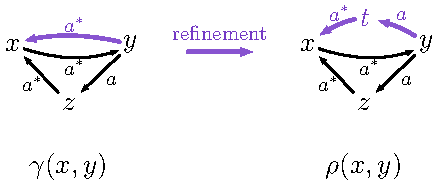
\includegraphics[width=.45\linewidth]{fig/prelim-db/basic-refinement.pdf}
    }
    \hfill
    \subfloat[\AP\label{fig:basic-hom}A "strong onto homomorphism" between "CRPQs".]{
        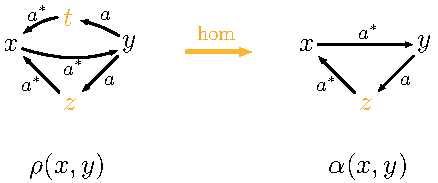
\includegraphics[width=.45\linewidth]{fig/prelim-db/basic-hom.pdf}
    }
	\caption{"Homomorphisms" and "refinements" between "CRPQs".}
\end{figure}
By convention, $t \atom{a^{-}} t'$ is a shorthand for $t' \atom{a} t$. As a consequence,
the underlying graph of an "atom $m$-refinement" of the form \eqref{eq:refinement} is not necessarily a directed path.
By definition, note that
$L_1\cdots L_n \subseteq L$ and hence $\rho \contained \gamma$ for any "atom $m$-refinement" $\rho$ of $\gamma$.
An \AP""atom refinement"" is an "atom $m$-refinement" for some $m$.
An example is provided in \Cref{fig:basic-refinement}.

\begin{definition}
    \AP\label{def:atom-contraction}
    \AP Given an "atom refinement" $\rho = x \atom{L_1} t_1 \atom{L_2} \dotsc \atom{L_{n-1}} t_{n-1} \atom{L_n} y$ of $\gamma = x \atom{L} y$ as in \eqref{eq:refinement}, define
    a ""condensation"" of $\rho$ between $t_i$ and $t_j$, where $0 \leq i,j \leq n$ and $j > i+1$, as any "C2RPQ" of the form:
    \[
        \rho' = x \atom{L_1} t_1 \atom{L_2} \dotsc \atom{L_i} \textcolor{maincolor}{t_i \atom{K} t_j} \atom{L_{j+1}} \dotsc
        \atom{L_{n-1}} t_{n-1} \atom{L_n} y
    \]
    such that $\textcolor{maincolor}{K = \+A[q_i,q_j]}$.
	\begin{fact}
		\AP\label{fact:refinement-contained}
		Every "condensation" $\rho'$ of $\rho$ is a "refinement" of $\gamma$, and $\rho \contained \rho' \contained \gamma$.
	\end{fact}
    \AP Informally, we will abuse the notation and
    write $\intro*\contract{L_{i}\cdots L_{j}}$ to denote the language $K$---even if this language
    does not only depend on $L_{i}\cdots L_{j}$.
\end{definition}

\begin{example}
    \AP\label{ex:atom-refinement-twoway}
    Let $\gamma(x,y) = x \atom{(aa^-)^*} y$ be a "C2RPQ" "atom", where
    $(aa^-)^*$ is implicitly represented by its minimal automaton.
    Then $\rho(x,y)$ is a "refinement" of "refinement length" seven of $\gamma(x,y)$
    and $\rho'(x,y)$ is a "condensation" of $\rho(x,y)$, where:
    \begin{align*}
        \rho(x,y) & = x \atom{a} t_1 \atom{(a^-a)^*} t_2 \atom{(a^-a)^*} t_3
            \coatom{a} t_4 \atom{(aa^-)^*} t_5 \atom{(aa^-)^*a} t_6 \coatom{a} y, \\
        \rho'(x,y) & = x \atom{a} t_1 \atom{(a^-a)^*} t_2 \atom{(a^-a)^*} t_3
		\coatom{a} t_4 \atom{(aa^-)^*} y. 
    \end{align*}
    On the other hand, $\rho''(x,y) = x \atom{a} t_1 \coatom{a} y$ is not
    a "condensation" of $\rho(x,y)$.
\end{example}

Given a natural number $m$, an \AP""$m$-refinement"" of a "C2RPQ" $\gamma(\bar x) = \bigwedge_{i} x_i \atom{L_i} y_i$ is any query resulting from: (1) replacing every "atom" by one of its "$m$-refinements@@atom", and (2)
should some "$m$-refinements@@atom" have "equality atoms",
collapsing the variables.
\AP A ""refinement"" is an "$m$-refinement" for some $m$.
Note that any "atom $m$-refinements" is, by definition, also an
"atom $m'$-refinements" when $m \leq m'$: as a consequence, in the "refinement" of a "C2RPQ"
the "atom refinements" need not have the same length.
For instance, both $\rho(x,x) = x \atom{c} x$ and $\rho'(x,y) = x \atom{a} t_1 \atom{a} y \coatom{c} y$ are "refinements" of $\gamma(x,y) = x \atom{a^*} y \coatom{c} x$.

For a given "C2RPQ" $\gamma$, let $\AP\intro*\Refin[\leq m](\gamma)$ be the set of all "$m$-refinements" of $\gamma$, and $\reintro*\Refin(\gamma)$ be the set of all its "refinements".
Given a "refinement" $\rho(\bar x)$ of $\gamma(\bar x)$,
its ""refinement length"" is the least natural number
$m$ such that $\rho(\bar x) \in \Refin[\leq m](\gamma)$.
Note that if the automaton representing a language $L$ has more than one final state, for instance the minimal automaton for $L = a^+ + b^+$,
then $x \atom{L} y$ is not a "refinement" of itself.
However, it will always be "equivalent" to a union of refinements: in
this example, $x \atom{a^+ + b^+} y$ is "equivalent" to the union of
$x \atom{a^+} y$ and $x \atom{b^+} y$, which are both "refinements"
of the original "C2RPQ".

\paragraph*{Expansions.}
Remember that a "C2RPQ" whose languages are
of the form $\set{a}$ or $\set{a^-}$ for $a \in \A$ is in effect a "CQ".
The \AP""expansions"" of a "C2RPQ" $\gamma$ is the set $\intro*\Exp(\gamma)$ of all "CQs" which are "refinements" of $\gamma$.
In other words, an "expansion" of $\gamma$ is any "CQ" obtained from $\gamma$
by replacing each "atom" $x \atom{L} y$ by a path $x \atom{w} y$ for some
word $w \in L$.
For instance, $\xi(x,y) = x \atom{a} t_1 \coatom{a} t_2 \atom{a} t_3 \coatom{a} y$
is an "expansion" of $\rho(x,y) = x \atom{(aa^-)^*} y$.
\begin{marginfigure}[-4em]
    \centering
    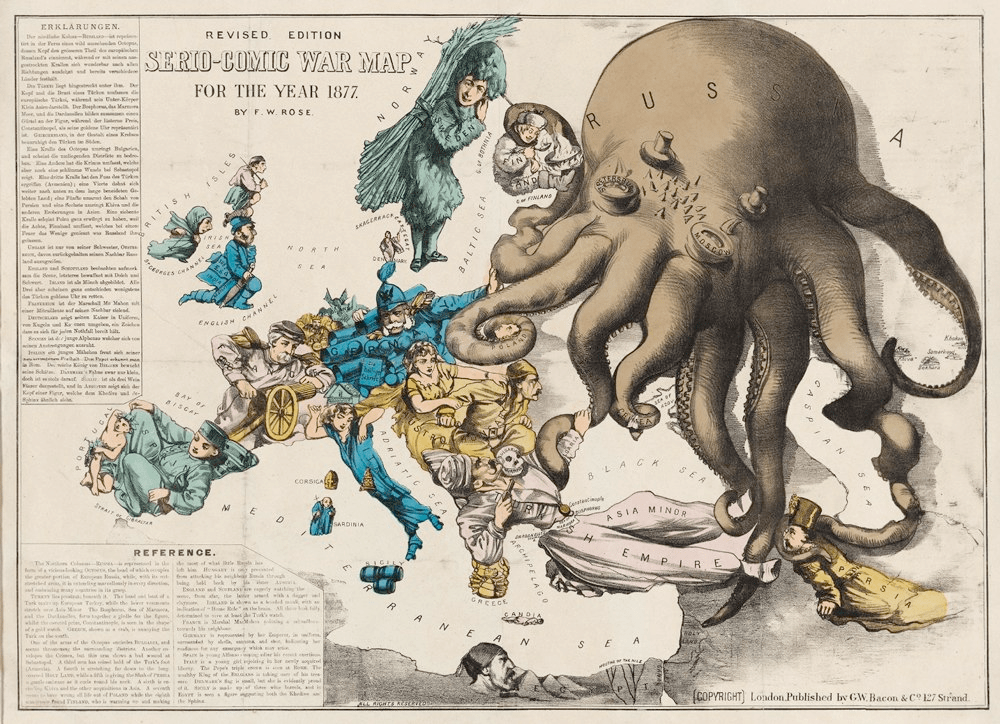
\includegraphics[width=\linewidth]{fig/prelim-db/Russia.png}
    \caption{\emph{Serio-comic war map for the year 1877}, by F. W. Rose.}
\end{marginfigure}

\paragraph{Canonical databases.}
We define the \AP""canonical databases@@CRPQ"" of a "C2RPQ" as the "canonical databases@@CQ"
of the "expansions" of the "query@C2RPQ". We denote by
\AP$\tup{\?G,\bar u} \intro*\cdb \gamma(\bar x)$
the fact that $\tup{\?G,\bar u}$ is a "canonical database@@CRPQ" of $\gamma(\bar x)$.
We extend the notions of "expansions" and of "canonical databases" to "UC(2)RPQs" by
taking the union.

Notice that any "UC2RPQ" is equivalent to the infinitary union of its "expansions". In light of this, the semantics for "UC2RPQ" can be rephrased as follows. 
Given a "UC2RPQ" $\Gamma(\bar x)$ and a graph database $\?G$, 
the "evaluation" of $\Gamma(\bar x)$ over $\?H$, is the set of tuples 
$\bar{v}$ of nodes for which:
\begin{itemize}
    \item there is $\anexpansion \in \Exp(\Gamma)$ such that there is an "evaluation map" from $\anexpansion$ to $\?H$ that sends $\bar x$ onto $\bar v$, or equivalently
    \item there exists $\tup{\?G, \bar u} \cdb \Gamma(\bar x)$ "st"
    $\tup{\?G, \bar u} \homto \tup{\?H, \bar v}$.
\end{itemize}
In this specific case, since $\anexpansion$ is a "CQ", the notion of "evaluation map"
coincides with that of "homomorphism":
"duality@@CQ" justifies that we use these two notions interchangeably, which we will
happily do from now on.

Similarly, "containment" of "UC2RPQs" can also be characterized in terms of "expansions".
\begin{proposition}[Folklore]
    \!\footnote{The proof is elementary,
    see "eg" \cite[Proposition 3.2]{FlorescuLevySuciu1998Containment} 
    or \cite[Theorem 2]{CalvaneseDeGiacomoLenzeriniVardi2000Containment}.}
    \footnote{The proposition works for "Boolean" as well as "non-Boolean" queries:
    we dropped the tuples of variables for the sake of readability.}
    \AP\label{prop:cont-char-exp-st}
    Let $\Gamma_1$ and $\Gamma_2$ be "UC2RPQs". The following are equivalent:
    \begin{itemize}
        \item $\Gamma_1 \contained \Gamma_2$;
        \item for every $\anexpansion_1\in \Exp(\Gamma_1)$, we have $\anexpansion_1 \contained \Gamma_2$;
        \item for every $\anexpansion_1\in \Exp(\Gamma_1)$ there exists $\anexpansion_2\in \Exp(\Gamma_2)$ such that $\anexpansion_2\homto \anexpansion_1$;
        \item for every $\?G_1 \cdb \Gamma_1$, we have $\?G_1 \FOmodels \Gamma_2$;
        \item for every $\?G_1 \cdb \Gamma_1$, there exists $\?G_2 \cdb \Gamma_2$
        "st" $\?G_2 \homto \?G_1$;
    \end{itemize}
\end{proposition}

\begin{marginfigure}
    \centering
    \begin{tikzpicture}
        \node[vertex] (0) at (0,0) {};
        \node[vertex,right=1cm of 0] (1) {};
        \node[vertex,right=1cm of 1] (2) {};
        \node[vertex,right=1cm of 2] (3) {};
        \node[vertex,below right = 1.5cm and .5cm of 0] (a) {};
        \node[vertex,right =1cm of a] (b) {};
        \node[vertex,right =1cm of b] (c) {};
        \draw[edge] (0) edge node[above] {$a$} (1)
            (1) edge[cRed] node[above, cRed] {$a$} (2)
            (2) edge node[above] {$b$} (3)
            (a) edge node[above] {$a$} (b)
            (b) edge node[above] {$b$} (c);
        \draw[edge, dotted] (a) edge[out=90,in=-90] (1)
            (b) edge[out=90,in=-90] (2)
            (c) edge[out=90,in=-90] (3);
    \end{tikzpicture}
    \caption{\AP\label{fig:ex-containment-non-uniform-a} "Homomorphism"
    from $\?D$ to $\?G_a$.}
\end{marginfigure}
\begin{marginfigure}
    \centering
    \begin{tikzpicture}
        \node[vertex] (0) at (0,0) {};
        \node[vertex,right=1cm of 0] (1) {};
        \node[vertex,right=1cm of 1] (2) {};
        \node[vertex,right=1cm of 2] (3) {};
        \node[vertex,below right = 1.5cm and .5cm of 0] (a) {};
        \node[vertex,right =1cm of a] (b) {};
        \node[vertex,right =1cm of b] (c) {};
        \draw[edge] (0) edge node[above] {$a$} (1)
            (1) edge[cBlue] node[above, cBlue] {$b$} (2)
            (2) edge node[above] {$b$} (3)
            (a) edge node[above] {$a$} (b)
            (b) edge node[above] {$b$} (c);
        \draw[edge, dotted] (a) edge[out=90,in=-90] (0)
            (b) edge[out=90,in=-90] (1)
            (c) edge[out=90,in=-90] (2);
    \end{tikzpicture}
    \caption{\AP\label{fig:ex-containment-non-uniform-b} "Homomorphism"
    from $\?D$ to $\?G_b$.}
\end{marginfigure}

As an example, we consider the queries
\[
    \gamma() \defeq w \atom{a} x \atom{a+b} y \atom{b} z
    \quad\text{and}\quad 
    \delta() \defeq x \atom{a} y \atom{b} z
\]
from \Cref{ex:ex-containment-non-uniform}.
Then $\delta()$ has a unique "canonical database@@CRPQ" that we denote
by $\?D$, and $\gamma()$ has two "canonical databases@@CRPQ" 
$\?G_a$ and $\?G_b$. We represent them in \Cref{fig:ex-containment-non-uniform-a,fig:ex-containment-non-uniform-b},
together with witnesses that $\gamma() \contained \delta()$.

\Cref{prop:cont-char-exp-st} by itself is not enough to conclude to the decidability of
"containment" since the set of "expansions" or "canonical databases@@CRPQ"
of a "UC2RPQ", or even simply "CRPQs", is infinite.
To get decidability, the easiest way is by proving a small model property.
\begin{proposition}[Small model property for C2RPQs, folklore]
    \label{prop:pigeonssssssss}
    Given two "C2RPQs" $\gamma_1(\bar x_1)$ and $\gamma_2(\bar x_2)$, if $\gamma_1(\bar x_1) \notcontained \gamma_2(\bar x_2)$, then there exists $\tup{\?G_1, \bar u_1} \cdb \gamma_1(\bar x_1)$ of size at most $f(\size{\gamma_1}+\size{\gamma_2})$ "st"
    $\tup{\?G_1, \bar u_1} \notFOmodels \gamma_2(\bar x_2)$,
    where $f$ is a doubly-exponential function.
\end{proposition}

\begin{proof}[Proof sketch]
    We start with some $\tup{\?G_1, \bar u_1} \cdb \gamma_1(\bar x_1)$ of arbitrary size
    such that $\tup{\?G_1, \bar u_1} \notFOmodels \gamma_2(\bar x_2)$.
    On then look at how $\gamma_2$ maps into $\?G_1$ in the following sense:
    in an "atom refinement" in $\?G_1$
    \[
        x_0 \atom{a_1} x_1 \atom{a_2} \dotsc \atom{a_n} x_n
    \]
    we associate to every sequence $a_1 a_{2} \cdots a_i$ the function
    which takes a tuple of set of automaton states (one set for each automaton of $\gamma_2$),
    and returns the tuple of set of states they can reach after reading $a_i a_{i+1} \cdots a_j$.
    By pigeon-hole principle, if $n$ has at least double-exponential size, then there must exist
    two indices $i < j$ that have the same behaviour.
    Then, shrinking \[
        x_0 \atom{a_1} x_1 \atom{a_2} \dotsc \atom{a_n} x_n
    \quad\text{into}\quad
        x_0 \atom{a_1} x_1 \atom{a_2} \dotsc \atom{a_i} x_i = x_j \atom{a_{j+1}} \dotsc \atom{a_n} x_n
    \]
    yields a strictly smaller "canonical database" $\?G'_1$ of $\gamma_1$
    that behaves like $\?G_1$ "wrt" to the automata of $\gamma_2$,
    and so since we had $\tup{\?G_1, \bar u_1} \notFOmodels\ \gamma_2(\bar x_2)$,
    we still have $\tup{\?G'_1, \bar u_1} \notFOmodels\ \gamma_2(\bar x_2)$.
\end{proof}
\begin{marginfigure}[-15em]
    \centering
    
\includegraphics[width=\linewidth]{fig/prelim-db/pigeon.jpg}
    \caption{Fun interlude: try spotting the difference with \Cref{prop:pigeonssssssss}.
    \href{https://commons.wikimedia.org/wiki/File:Spinifex\_Pigeon\_0A2A1585.jpg}{\emph{Spinifex Pigeon}}, by JJ Harrison, licensed under "CC BY SA 3.0".}
\end{marginfigure}

In particular \Cref{prop:pigeonssssssss} implies that "containment" is decidable
for "UC2RPQs". However, this does not give an optimal algorithm.

\begin{proposition}
    \!{Proven independently in \cite[Theorem 5]{CalvaneseDeGiacomoLenzeriniVardi2000Containment} for "C2RPQs"
    and in \cite[§ after Theorem 4.8]{FlorescuLevySuciu1998Containment} for "CRPQs" without 
    inverses but with an infinite alphabet.}
    \label{prop:containment-expspace-complete}
    Containment of "UC2RPQs" is "ExpSpace"-complete. The lower bound already
    holds for "Boolean CRPQs".
\end{proposition}

Overtime, this proof has been simplified to eventually climax
to the following result.
\begin{proposition}[{\cite[Lemma 8]{Figueira2020Containment}}]
	\AP\label{prop:containment-figueira}
	There is a fixed alphabet over which the
	"con\-tainment problem" for "Boolean CRPQs" is already "ExpSpace"-hard
    when restricted
	to instances of the form
	\begin{center}
		\begin{tikzcd}[column sep=scriptsize]
			\hphantom{\quad\textnormal{where:}}
			\gamma_1() = \qvar \rar["K"] & \qvar & \contained^{?} & 
			\qvar \rar["L_1", bend left=40] \rar["\raisebox{6pt}{\small\vdots}", phantom] \rar["L_p" below, bend right=40] & \qvar &[-2.1em] = \gamma_2().
		\end{tikzcd}
	\end{center}
\end{proposition}

Observe that, while the "containment"
\[
(\gamma_1(x,y) \defeq x \atom{K} y)
\contained^? 
(\gamma_2(x,y) \defeq x \atom{L} y)
\]
is equivalent to $K \contained^? L$,
we have that 
\[
(\gamma_1() \defeq x \atom{K} y)
\contained^? 
(\gamma_2() \defeq x \atom{L} y)
\]
is rather equivalent to $K \contained^? \A^* L \A^*$,
and so the problem of \Cref{prop:containment-figueira}
can be reformulated as
\[
    K \subseteq^? \A^* \big( \bigcap_{i=1}^p L_i \big) \A^*.
\]
The proof of \Cref{prop:containment-figueira} is by reduction
from the exponential-space tiling problem,
and relies on encoding exponential-sized counters in polynomial space.

\paragraph*{Hom-Minimality.}
We say that a "graph database" $\tup{\?G,\bar u}$ satisfying a ""semantical query"" $\gamma(\bar x)$
is \AP""hom-minimal"" if for every other "graph database" $\tup{\?G',\bar v}$,
if $\tup{\?G',\bar v}$ also satisfies $\gamma(\bar x)$ and
if $\tup{\?G', \bar v} \homto \tup{\?G, \bar u}$ then $\tup{\?G', \bar v} \semequiv \tup{\?G, \bar u}$. Graphically, this literally corresponds to the minimal elements of a set in
\Cref{fig:distributive-lattice-rel-db}.
In the definition, the quantification over all ``$\tup{\?G',\bar v}$ that satisfy $\gamma(\bar x)$''
can actually be replaced, for "UC2RPQs", by a quantification over all "canonical databases".

\subsection{Queries Over Simple Languages}

The high complexity of \Cref{prop:containment-figueira,prop:variation-figueira-simple} motivate
the quest for fragments of "conjunctive regular path queries" with better complexity.
We will present a fragment {\UCRPQSRE} that
has a "containment problem" that is much better behaved than for general "UCRPQs",
and moreover is widely used in practice.

\AP A ""simple regular expression"", or \reintro{SRE}, is a regular expression the form $a^*$ for some letter $a \in \A$ or of the form $a_1 + \dotsb + a_m$ for some $a_1, \dotsc, a_m \in \A$. 
\AP Let \intro*{\UCRPQSRE} be the set of all "UCRPQ" whose languages are expressed via "simple regular expressions". Observe that {\UCRPQSRE} is "semantically equivalent" to the class of "UCRPQs" over the closure under concatenation of "simple regular expressions"
since $\gamma(x,y) = x \atom{e_1 \cdot e_2} y$ is equivalent to $\gamma'(x,y) = x \atom{e_1} z \land  z \atom{e_2} y$.
Moreover, \UCRPQSRE{} also corresponds to "UC2RPQ" whose languages are expressed via "SREs";
in other words adding two-wayness does not increase the expressivity of the class. 

\begin{proposition}[{\cite[Corollary 5.2]{FigueiraEtal2020Containment}}]
    "Containment" of {\UCRPQSRE} is "PiP2"-complete.
\end{proposition}

In other words, this problem is just one level up the polynomial hierarchy compared to the "CQ" "containment problem", which sharply contrasts with the costly "ExpSpace"-completeness result
for the full class of "UC2RPQs"!
Moreover, recent studies on SPARQL query logs on Wikidata, DBpedia and other sources show that this kind of regular expressions cover a majority of the queries investigated, "eg", 75\% of
the ``property paths'' ("C2RPQ" "atoms") of the corpus of 1.5M queries of Bonifati, Martens and Timm \cite[Table 15]{BonifatiMartensTimm2020SPARQL}.

In \Cref{ch:minimization-CRPQ} we will actually need a marginally smaller subclass of these:
we define \AP""positive simple regular expressions"" analogously to
"simple regular expressions" but by replacing $a^*$ with $a^+$.

\subsection{Static Analysis}

Static optimization for CRPQs has received considerable attention. Beyond the basic study of containment and equivalence problems for CRPQs that we already mentioned,
let us highlight that
these problems have also been investigated under different scenarios: restrictions on the shape of queries \cite{Figueira2020Containment}, restrictions on their regular languages \cite{FigueiraEtal2020Containment}, alternative semantics~\cite{FigueiraRomero23}, or under schema information~\cite{GutierresBasultoGutowskiIbanezGarciaMurlak2022Finite,GutierresBasultoGutowskiIbanezGarciaMurlak2024Containment}.
This has enabled the study of more advanced static analysis problems motivated by the following general question: \emph{Can a given query be equivalently rewritten as one from a target fragment (which enjoys desirable properties)?}
In the literature the problem has been studied where the target fragment are queries which either (i) avoid having infinite languages, or (ii) have a tree-like structure. This gives rise to the so-called (i) \emph{boundedness problem} for CRPQs ("ie", whether a CRPQ is equivalent to a UCQ) \cite{BarceloFigueiraRomero2019Boundedness,FigueiraKrishnaSwostikMishraPadmanabha2024Boundedness}, and (ii) \emph{semantic treewidth problem} for CRPQs ("ie", whether a CRPQ is equivalent to one 
that is tree-shaped) \cite{BarceloRomeroVardi2016SemanticAcyclicity}.

In the next chapters,
we focus on the problems of minimizing the number of "atoms"
(\Cref{ch:minimization-CRPQ}) and "tree-width" (\Cref{ch:minimization-CRPQ})
necessary to express a "(U)C(2)RPQ". In both cases,
we will prove decidability of the problem by providing an algorithm in
"$k$-ExpSpace" for some $k$, and will provide a much more efficient algorithm---"ie" in the
polynomial hierarchy---for queries over "simple regular expressions".


% \todo{fixed nb languages}

% \subsection{Beyond Conjunctive Regular Path Queries}

% \todo{}
% - extended CRPQs

% - sql + recursion ()

% - mso

% - datalog / monadic / linear

% \subsection{Analysis of Conjunctive Regular Path Queries}

% \todo{}
% small intro of the next two chapters
% + brief litterature review (ex: bridgewidth)